\begin{figure}[htp]
  \centering
  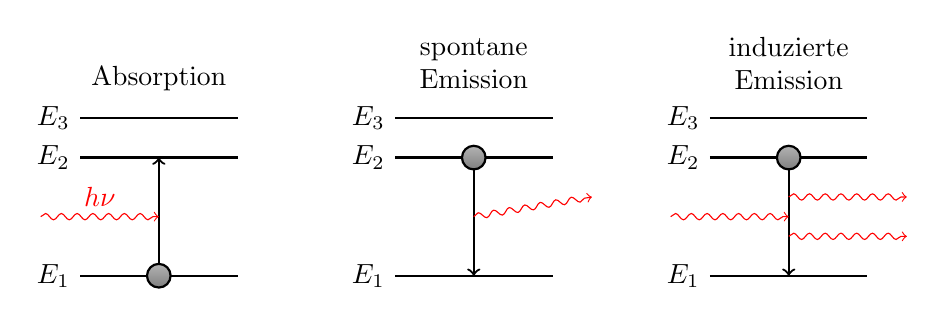
\begin{tikzpicture}[every text node part/.style={align=center}]
    \draw[thick] (-1,0)node[left]{$E_1$} -- (1,0);
    \draw[thick] (-1,1.5)node[left]{$E_2$} -- (1,1.5);
    \draw[thick] (-1,2)node[left]{$E_3$} -- (1,2);
    \node (A) at (0,2.5){Absorption};
    \draw[thick, ->] (0,0) -- (0,1.5);
    \draw[->,red, decorate, decoration={snake,amplitude=.4mm,segment length=2mm,post length=0.5mm}] (-1.5,.75) --node[above]{$h\nu$} (0,.75);
    \shadedraw[draw=black, thick, top color = black!30!white, bottom color=black!50!white] (0,0) circle (.15cm);

    \begin{scope}[shift={(4,0)}]
      \draw[thick] (-1,0)node[left]{$E_1$} -- (1,0);
      \draw[thick] (-1,1.5)node[left]{$E_2$} -- (1,1.5);
      \draw[thick] (-1,2)node[left]{$E_3$} -- (1,2);
      \node (A) at (0,2.7){spontane\\Emission};
      \draw[thick, <-] (0,0) -- (0,1.5);
      \draw[->,red, decorate, decoration={snake,amplitude=.4mm,segment length=2mm,post length=0.5mm}] (0,.75) -- (1.5,1);
      \shadedraw[draw=black, thick, top color = black!30!white, bottom color=black!50!white] (0,1.5) circle (.15cm);
    \end{scope}

    \begin{scope}[shift={(8,0)}]
      \draw[thick] (-1,0)node[left]{$E_1$} -- (1,0);
      \draw[thick] (-1,1.5)node[left]{$E_2$} -- (1,1.5);
      \draw[thick] (-1,2)node[left]{$E_3$} -- (1,2);
      \node (A) at (0,2.7){induzierte\\Emission};
      \draw[thick, <-] (0,0) -- (0,1.5);
      \draw[->,red, decorate, decoration={snake,amplitude=.4mm,segment length=2mm,post length=0.5mm}] (-1.5,.75) -- (0,.75);
      \draw[->,red, decorate, decoration={snake,amplitude=.4mm,segment length=2mm,post length=0.5mm}] (0,1) -- (1.5,1);
      \draw[->,red, decorate, decoration={snake,amplitude=.4mm,segment length=2mm,post length=0.5mm}] (0,.5) -- (1.5,.5);
      \shadedraw[draw=black, thick, top color = black!30!white, bottom color=black!50!white] (0,1.5) circle (.15cm);
    \end{scope}
  \end{tikzpicture}
  \caption{Schematische Darstellung von Absorptions- und Emissionsprozessen nach~\cite{Eichler}.}
  \label{fig:Absorption_Emission}
\end{figure}
